\chapter{Projeto do Comitê de Ética} \label{sec:comite}
\section{Resumo}
Com os recentes avanços na tecnologia de sensores sem fio, é possível incorporá-los na roupa ou no corpo (\textit{wearable}) do usuário e isso proporciona uma monitorização contínua dos sinais vitais. Contudo a concepção de um sistema de monitoramento \textit{wearable} que não seja invasivo ainda é um grande desafio. Por outro lado, a necessidade de integrar diferentes sensores em uma única solução dificulta essa atividade, pois os dispositivos são considerados pesados, visíveis e estereotipados pelos próprios usuários ~\cite{aarhus_negotiating_2010}, por esse motivo esses dispositivos são refutados, inviabilizando o monitoramento contínuo da saúde nesses casos. Contudo, desde 2005 os jogos eletrônicos fazem uso de dispositivos como acelerômetros, giroscópio, dispositivos de captura de movimento possibilitando ao usuário estivesse uma maior imersão no universo do jogo através da análise de seus movimentos. Esses sensores usados em jogos eletrônicos permitem capturar sinais  de tremores ~\cite{synnott_wiipd_2012,lemoyne2010} 
e posturais que são sintomas presentes no \ac{dp}. Como o uso desses dispositivos já está embutido no contexto do jogo, possivelmente o usuário não iria sentir desconforto caso fossem usados para monitorar os sintomas do \ac{dp} enquanto estivesse num momento de descontração ao usar um jogo eletrônico. 

\section{Introdução}
A \ac{dp} é uma das doenças mais comum nos idosos. Apesar dos sintomas clássicos o diagnóstico clínico não é específico, não há exames laboratoriais, diagnósticos e existem outras doenças que se manifestam como o \ac{dp} ~\cite{vedolin2003,tolosa06}. O \ac{dp} é uma afecção do sistema nervoso central, a qual é expressa de forma crônica e progressiva. Ela é causada pela degeneração dos neurônios produtores de dopamina presente na substância negra e caracterizada pelos sintomas parkinsonianos: tremor em repouso (que diminui durante movimentos voluntários); bradicinesia ou hipocinesia (lentidão e escassez de movimentos, além de dificuldade na marcha), rigidez muscular (aumento da resistência ao movimento passivo dos membros), perda de reflexos posturais que leva a alteração da marcha e aumenta a ocorrência de queda ~\cite{tolosa06,rodrigues2006}. 

Parkinsonismo é um termo genérico que designa uma série de doenças com causas diferentes e que têm em comum a presença de sintomas frequentemente encontrados no~\ac{dp}. Esta doença é uma das muitas formas de parkinsonismo, correspondendo a cerca de 75$\%$ dos casos. A evolução da doença a gravidade e a progressão dos sintomas variam de um paciente para outro. No momento não existe teste diagnóstico para a doença e estudos comprovam dificuldade na diferenciação clínica entre \ac{dp} e outras formas de parkinsonismo. A maioria dos neurologistas concorda que o diagnóstico do \ac{dp} requer a identificação de alguma combinação de sinais motores cardinais (tremor de repouso, bradicinesia, rigidez tipo roda denteada, alterações posturais), porém uma classificação clínica padrão ainda não foi obtida ~\cite{protpar010}. Além do mais, um diagnóstico auxiliar importante é a resposta dos pacientes aos medicamentos antiparkinsonianos tal como a levodopa ~\cite{protpar010}. Os pacientes com~\ac{dp} quase 
sempre apresentam uma resposta satisfatória a esse medicamento, e no caso de não responder satisfatoriamente à levodopa, é provável que o diagnóstico seja de outra forma de parkinsonismo. Porém, na literatura ~\cite{rowlandtratado} uma resposta à levodopa não confirma o diagnóstico do \ac{dp} porque existem muitos casos de parkinsonismo sintomático e muitas formas de síndrome de Parkinson em seus estágios iniciais que também respondem à levodopa. 

O \ac{dp} é uma doença mais comum em idosos, porém existem casos precoces de início da doença em indivíduos antes dos 40 anos ou até mesmo abaixo dos 21 ~\cite{menezes2003}. A incidência da doença é estimada de 100 a 200 casos por 100.000 habitantes, com o avanço da idade a probabilidade do desenvolvimento da doença tende a aumentar. Por se tratar de uma doença progressiva, sua evolução acarreta em incapacidade grave após 10 a 15 anos, ocasionando em impacto social e financeiro, principalmente na população mais idosa. Estima-se que o custo anual mundial com medicamentos antiparkinsonianos esteja em torno de 11 bilhões de dólares, sendo o tratamento cerca de 3 a 4 vezes mais caro para pacientes na fase avançada da doença ~\cite{protpar010}.

Com o surgimento do tratamento para o \ac{dp} torna possível manter uma boa mobilidade funcional durante anos e aumenta a expectativa de vida dos pacientes tratados ~\cite{rodrigues2006}. Os fármacos do grupo dos antiparkinsonianos como a levodopa permitiram restaurar a atividade dopaminérgica que pode se encontrar reduzida, desta forma as drogas utilizadas são bem sucedidas no alívio de sintomas característicos da doença. Entretanto, devido aos efeitos colaterais frequentes induzidos pelos fármacos, é preciso iniciar o tratamento com esses medicamentos somente quando os sintomas estiverem prejudicando o desempenho profissional ou das atividades diárias do paciente ~\cite{rodrigues2006}.

A natureza progressiva do \ac{dp} e suas manifestações clínicas (motoras e não motoras),  associadas a efeitos colaterais precoces e tardios da intervenção terapêutica, tornam o tratamento da doença bastante complexo ~\cite{protpar010} e estima-se que a taxa de morte dos neurônios dopaminérgicos da substância negra situa-se  ao redor de 10$\%$ ao ano~\cite{national2006parkinson}. Consequentemente, com o passar do tempo a sintomatologia parkinsoniana piora necessitando aumentar as doses da medicação, logo com a progressão da doença, a eficácia do tratamento diminui e os pacientes passam a não responder ao tratamento medicamentoso ~\cite{protpar010}. 

Alternar entre os estados \textit{on} (``normal'') e \textit{off} (``com os sintomas parkisonianos''). As mudanças dos estados \textit{on} para \textit{off} dependerá do horário da ingestão do medicamento que tornará previsível a mudança para o estado \textit{on}. Contudo, alguns pacientes podem ter mudanças abruptas para o estado \textit{off}, sem qualquer correlação com o tempo em que a medicação foi ingerida. Essa irregularidade de não conseguir determinar o momento em que o paciente entrará no estado \textit{on} ou \textit{off} impacta diretamente nas avaliações objetivas do profissional que irá avaliar a evolução da doença ~\cite{kostek12,patel_monitoring_2009}. 

Outro efeito colateral no uso do medicamento bastante conhecido é o surgimento da discinesia (movimentos involuntários de contorção) em 80$\%$ dos pacientes que recebem a levodopa como tratamento prolongado. Esse sintoma pode ser aliviado com a diminuição da dose, por outro lado, os sintomas da doença tendem a retornar. Com o surgimento de discinesia intensa é necessário otimizar o gerenciamento do tratamento medicamentoso, levando a adicionar novos medicamentos para reduzir os sintomas incapacitantes a longo prazo ~\cite{rodrigues2006}. 

A partir dos tratamentos para o \ac{dp}, foram criadas escalas de avaliação do progresso da doença ~\cite{updrs87,Hoehn_Yahr_2001}. Essas escalas permitem avaliar: a condição clínica geral, incapacidades, funções motoras e mentais e até mesmo a qualidade de vida dos pacientes. Esses instrumentos são importantes tanto no nível clínico quanto no científico, pois permitem monitorar a progressão da doença e a eficácia do tratamento medicamentoso ~\cite{updrs87,goul05}.  Sendo assim, foi criada em 1987 a Escala Unificada de Avaliação da  Doença de Parkinson (Unified Parkinson’s Disease Rating Scale – UPDRS) ~\cite{updrs87} que é amplamente utilizada para monitorar a progressão da doença e a eficácia do tratamento, sendo considerada confiável, válida e qualificada como um método adequado para a avaliação do~\ac{dp} ~\cite{goul05}. 

% 
% Atualmente a evolução da \ac{dp} é avaliada através de escalas, que permitem avaliar a eficácia do tratamentos e sua aplicabilidade nas práticas fisioterápicas. Segundo um trabalho de Goulart ~\cite{goul05} as escalas de estágios de incapacidade representadas por Hoehn/Yahr ~\cite{Hoehn_Yahr_2001} e a UPDRS ~\cite{updrs87} são consideradas as de maior confiabilidade, podendo ser usadas por fisioterapeutas para melhor avaliação do estado clínico-funcional do  paciente.

Na UPDRS a evolução do~\ac{dp} é classificada nas seguintes fases ~\cite{updrs87}:
  \begin{itemize}
    \item \textbf{ESTÁGIO 0:} Nenhum sinal da doença;
    \item \textbf{ESTÁGIO 1:} Doença unilateral;
    \item \textbf{ESTÁGIO 1,5:} Envolvimento unilateral e axial;
    \item \textbf{ESTÁGIO 2:} Doença bilateral sem déficit de equilíbrio;
    \item \textbf{ESTÁGIO 2,5:} Doença bilateral leve, com recuperação no “teste do empurrão”;
    \item \textbf{ESTÁGIO 3:} Doença bilateral leve a moderada; alguma instabilidade postural; capacidade para viver independente;
    \item \textbf{ESTÁGIO 4:} Incapacidade grave, ainda capaz de caminhar ou permanecer de pé sem ajuda;
    \item \textbf{ESTÁGIO 5:} Confinado à cama ou cadeira de rodas a não ser que receba ajuda.
  \end{itemize}

A UPDRS é composta por 42 itens, divididos em quatro partes (atividade mental, comportamento e humor, atividades de vida diária e exploração motora e complicações da terapia medicamentosa) e através da avaliação desses sintomas, por intermédio do auto-relato e da observação clínica, é possível classificar em que estágio da doença o paciente se encontra. Contudo, justamente por ser baseada em auto-relato e observação clínica a qual é realizada eventualmente com a presença de um profissional, pesquisadores questionam a efetividade da avaliação do estágio da doença e propõem alternativas para avaliação dos itens motores de forma quantitativa através de sensores, os quais permitem monitorar o estágio do paciente ~\cite{kostek12,synnott_wiipd_2012,patel_monitoring_2009}.


A identificação dos sintomas do \ac{dp} durante a rotina diária permite um diagnóstico mais precoce da doença e consequentemente obter seus benefícios de um tratamento mais duradouro. Além disso, o monitoramento dos efeitos da medicação usada pelo paciente permite um gerenciamento da medicação e consequentemente reduz os sintomas indesejáveis da doença e prolongando a qualidade de vida do paciente.

Com os recentes avanços na tecnologia de sensores sem fio, é possível incorporá-los na roupa ou no corpo (\textit{wearable}) do usuário e isso proporciona uma monitorização contínua dos sinais vitais. Contudo a concepção de um sistema de monitoramento \textit{wearable} que não seja invasivo ainda é um grande desafio ~\cite{alemdar}. Por outro lado, a necessidade de integrar diferentes sensores em uma única solução dificulta essa atividade, pois os dispositivos são considerados pesados, visíveis e estereotipados pelos próprios usuários ~\cite{aarhus_negotiating_2010}, por esse motivo esses dispositivos são refutados, inviabilizando o monitoramento contínuo da saúde nesses casos. Contudo, desde 2005 os jogos eletrônicos fazem uso de dispositivos como acelerômetros, giroscópio, dispositivos de captura de movimento possibilitando ao usuário estivesse uma maior imersão no universo do jogo através da análise de seus movimentos. Como visto na literatura científica, esse sensores usados em jogos eletrônicos permitem 
capturar sinais de tremores~\cite{synnott_wiipd_2012,lemoyne2010} e posturais que são sintomas presentes no \ac{dp}. Como o uso desses dispositivos já está embutido no contexto do jogo, possivelmente o usuário não iria sentir desconforto caso fossem usados para monitorar os sintomas do \ac{dp} enquanto estivesse num momento de descontração ao usar um jogo eletrônico. 

Os jogos eletrônicos não são usados somente por crianças e adolescente, em uma pesquisa da Entertainment Software Association, associação formada pelas principais fabricantes americanas de jogos eletrônicos \textit{``Essential Facts About the Computer and Video Game Industry"}~\cite{esa2011} demonstra que em 2011 os jogadores de videogame dos Estados Unidos possuem, em média, 37 anos e 29$\%$ dos jogadores de videogame possuem mais de 50 anos. Logo, temos uma parcela bastante significativa de usuários que podem ser beneficiados com o monitoramento de dados de saúde por intermédio dos jogos eletrônicos.

%fazer a figura
Como visto, o objetivo principal deste trabalho é possibilitar meios de monitorar o usuário e tentar identificar sintomas do \ac{dp} em diferentes momentos do dia com o propósito de possibilitar um diagnóstico precoce e melhorar no gerenciamento da dosagem medicamentosa contribuindo para um prolongamento da qualidade de vida dos pacientes com \ac{dp}.

% 
\section{Problemática}
Alinhar a jogabilidade e a possibilidade de monitoramento dos dados de saúde não é uma tarefa trivial. Pois deve ser levado em consideração o uso dos dispositivos e pensar na execução de movimentos ou ações que permitam esse monitoramento. Os movimentos não podem ser repetitivos pois, levaria o usuário jogar por um curto período e como consequência abandonaria o monitoramento ~\cite{Suhonen:2008:SFE:1457199.1457204}. Para propor um jogo que consiga obter um monitoramento dos dados de saúde, deve ser realizado um estudo sobre quais os movimentos e ações que o usuário deve executar. Posteriormente, na posse dessas ações, deverá ser testada a execução dessas atividades e sua captura e possível classificação conforme os trabalhos já existentes que realizam essas atividades~\cite{Ballegaard:2008:HEL:1357054.1357336,albanese2012,bachlin_parkinsons_2009,visionbased2009,patel_monitoring_2009}. De posse dos movimentos e da captura dos dados será feito um levantamento de um \textit{game design} que permita executar os 
movimentos em  um ambiente lúdico e divertido como um jogo para entretenimento ~\cite{sweetser2005-gameflow}.


\section{Objetivo}
Essa pesquisa tem como objetivo identificar sintomas motores da doença de parkinson (tremores, bradicinesia e discinesia) através de um jogo eletrônico, dentro de um grupo de casos com doença de parkinson em diferentes estágios da doença segundo a UPDRS ~\cite{updrs87}.


\subsection{Específicos}
\begin{itemize}
 \item Capturar a  manifestação clínica de bradicinesia em casos de parkinson ao mover-se de um lado para o outro, levantar o braço e a perna através do uso de um dispositivo de captura de vídeo e reconhecimento de movimentos;
 \item Capturar os movimentos do grupo controle ao mover-se de um lado para o outro, levantar o braço e a perna através do uso de um dispositivo de captura de vídeo e reconhecimento de movimentos;
 \item Verificar a relação entre a manifestação do sintoma de bradicinesia em efeito com o medicamento antiparkinsoniano através do uso de um dispositivo de captura de vídeo e reconhecimento de movimentos;
\end{itemize}

\section{Material E Métodoo}

\subsection{Tipo de Estudo}
Estudo analítico de caso-controle.


\subsection{Local}
Grupo de pacientes da Clínica de Fisioterapia Dr. Rodrigo Ramalho pertencente ao Centro Universitário Cesmac.


\subsection{Amostra}
A técnica de amostragem utilizada para seleção, será por conveniência onde será composta por todos indivíduos que estejam diagnosticado com \ac{dp} e indivíduos da mesma faixa etária como grupo de controle.

\subsection{Formas de Recrutamento}
A forma de recrutamento deste protocolo será Circunscrita por intermédio de um profissional de saúde da própria Clínica de Fisioterapia. O profissional deverá conhecer a história clínica do paciente e obterá a permissão do mesmo para que a equipe de pesquisa possa entrar em contato.
A equipe de pesquisa deverá explicitar os riscos e benefícios da participação da pesquisa buscando a espontaneidade da decisão e depois fornecer o Termo De Consentimento Livre E Esclarecido.


\subsubsection{Critério de inclusão}
Casos com a \ac{dp} diagnosticada até o estágio 3 segundo a UPDRS ~\cite{updrs87}, sem distinção de sexo ou raça, que esteja com participação ativa na Clínica de Fisioterapia Dr. Rodrigo Ramalho e que aceitem participar do estudo.

\subsubsection{Critério de exclusão}
Pessoas com sintomas motores que não sejam do \ac{dp} e que tenham problemas em equilíbrio além daqueles que se neguem a participarem do estudo.

\subsection{Material}
Para a presente pesquisa serão testados dois jogos desenvolvidos por alunos do Instituto Federal de Alagoas (IFAL) e da Universidade Federal de Campina Grande (UFCG).

%\subsubsection{Jogo: Pinball World}
%O \textit{Pinball World}, é um jogo voltado para o entretenimento e pode ser usado por seus usuários em diferentes momentos do dia. O principal propósito do jogo é monitorar os sintomas de tremor das mãos do usuário por intermédio do acelerômetro usado como instrumento de controle. O usupário deverá movimentar o dispositivo para esquerda, direita e isso controlará a bola de \textit{pinball}, personagem principal do jogo. Durante o jogo o nível de tremor em movimento do usuário capturado e em outro momento em que o usuário precisa apenas visualizar o trajeto da bola, o jogador permanecerá parado e nesse momento será possível capturar o tremor de repouso. O jogo é composto por uma floresta e com  uma cachoeira e sua respectiva queda d'agua trazendo paz e tranquilidade ao jogador.
%
%O tremor de movimento é capturado durante os momentos em que o jogador precisa movimentar o dispositivo para controlar a bola e desviar de obstáculos. Em outro momento, quando o jogador mantém o dispositivo parado e precisa apenas visualizar o trajeto da bola, é possível capturar o tremor de repouso. As coordenadas do acelerômetro são capturadas a uma taxa de amostragem de 16Hz durante o curso do jogo. De acordo com a Tabela~\ref{tab:tremors}~\cite{albanese2012}, uma taxa de amostragem de 16Hz é suficiente para capturar os tipos de tremores que ocorrem nas mãos e membros. 
%
%
%\begin{figure}[!htb]
     %\centering
     %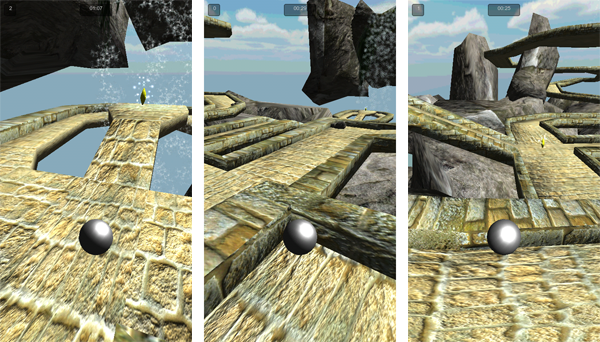
\includegraphics[scale=.6]{pinball_world.png}
     %\caption{O Jogo \emph{Pinball World}}
     %\label{img:pw1}
%\end{figure}
%
%\begin{table} 
%\centering 
%\caption{Tipos de tremor, diferenciados pela frequência, amplitude e início em relação a movimentos voluntários}
%\begin{center}
    %\begin{tabular}{ | l | p{2.5cm} | p{2.5cm} | p{2.5cm} | p{3.5cm} | }
        %\hline
        %Frequência & Tipo de tremor & Amplitude & Lado predominante & Relação com movimento voluntário \\ \hline
        %1-4 Hz & Cerebelar & Média-Alta & Membros & Postural, ação \\ \hline
        %3-5 Hz & Específico de tarefa & Baixa-Média & Mão & Escrita, segurar talheres, tocar instrumentos \\ \hline
        %4-5 Hz & Parkinsoniano & Média-Alta & Membros, mandíbula & Repouso \\ \hline
        %5-8 Hz & Essencial & Média-Alta & Membros, cabeça, voz & Postural \\ \hline
        %8-12 Hz & Fisiológico & Média & Membros & Postural \\ \hline
        %14-16 Hz & Ortostático & Baixa-Média & Pernas, tronco & Ficar de pé \\ \hline
    %\end{tabular}
%\end{center}
%\label{tab:tremors}
%\end{table}

\subsubsection{Jogo: \textit{Catch the Spheres}}
O jogo \textit{Catch the Spheres} é em terceira pessoa no qual o jogador, por meio de seu personagem, deverá capturar ou desviar de bolas que vêm em sua direção. Existem dois tipos de bolas: azuis e vermelhas. Inicialmente, todas as bolas são vermelhas e algumas destas mudam para a cor azul ao se aproximarem do jogador. O tempo para a bola mudar de cor pode ser menor ou maior, a depender do nível de dificuldade selecionado. Um personagem no centro do cenário replica todos os movimentos executados pelo jogador e capturado através do dispositivo de captura de vídeo. Deve-se tocar as bolas azuis com os pés ou as mãos e desviar das bolas vermelhas.

%\begin{figure}[!htb]
     %\centering
     %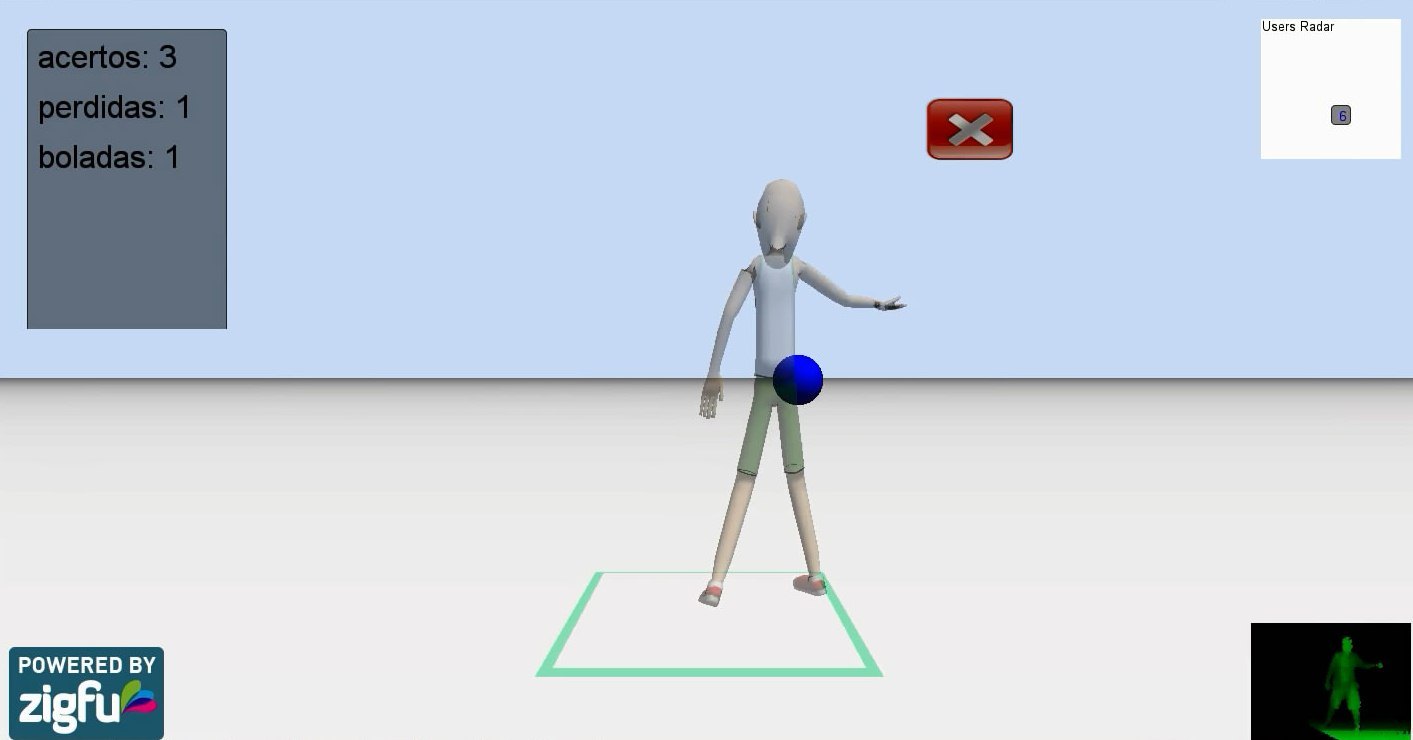
\includegraphics[width=.8\textwidth]{catch-the-spheres.jpg}
     %\caption{O jogo \emph{Catch the Spheres}}
     %\label{img:catch}
%\end{figure}

\begin{figure}[!htb]
     \centering
     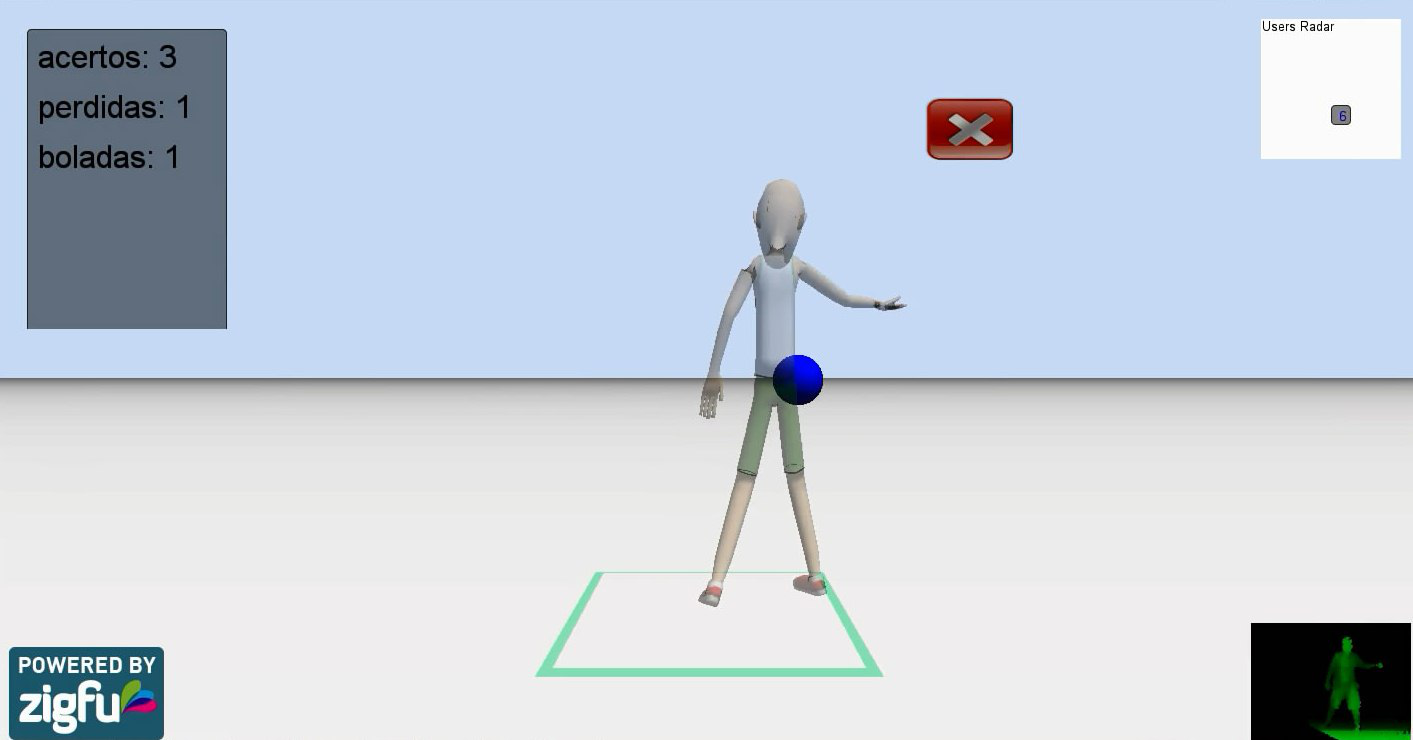
\includegraphics[width=.8\textwidth]{./img/catch-the-spheres.png}
     \caption{O jogo \emph{Catch the Spheres}}
     \label{img:catch}
\end{figure}

A finalidade do jogo é capturar dados do movimento do jogador enquanto ele executa as ações específicas do jogo. O intervalo de tempo entre o momento em que a bola muda de cor e o momento em que a bola é capturada pelo jogador mede o reflexo do jogador, enquanto que a velocidade dos seus membros é calculada através da distância percorrida pelas mãos ou pés para capturar as bolas.
Com a execução desse jogo, pretende-se colher dados para conseguir identificar os sintomas do \ac{dp} como bradicinesia.



\subsection{Procedimentos}

Este protocolo de pesquisa será submetido à avaliação do Comitê de Ética em Pesquisa do Centro Universitário Cesmac, somente depois da aprovação deste é que os dados serão coletados.

Para identificar a possibilidade de integrar o monitoramento da saúde do jogador por intermédio de jogos eletrônicos à sua rotina diária, será utilizada a abordagem \textit{Goal, Question, Metric} (GQM). GQM é uma abordagem hierárquica que inicia com objetivo principal e o divide em atividades que podem ser mensuradas durante a execução do projeto. É uma abordagem para integrar objetivos a modelos de processos de software, produtos e perspectivas de qualidade de interesse, baseado nas necessidades do projeto e da organização~\cite{van1999goal}. Os participantes da pesquisa serão convidados a responder o questionário GQM para avaliar se o jogo permite monitorar dados motores de forma não invasiva podendo estar integrado a rotina diária das pessoas.

%Os resultados que se desejam alcançar será o descobrimento de mecanismos para a identificação e classificação dos sintomas de tremores. O tremor é o principal sintoma parkinsoniano e a diferença dos ciclos pode auxiliar no diagnóstico da doença; sua maior frequência é quando o membro está em repouso sendo chamado de tremor de repouso.
Essa pesquisa também fará uma análise de jogos que fazem uso de sensores de movimento e avaliará as possibilidades de aquisição de dados de saúde baseada na Cinemática Angular do Movimento Humano. Através dos resultados obtidos pretendemos avaliar e classificar a normalidade e dificuldade na %execução de movimentos como levantar um braço, esticar uma perna ou balançar o corpo.
execução de movimentos como levantar um braço.

A coleta de dados será feita no próprio espaço sendo realizada em local reservado e de forma individual e permitindo sua participação por meio do Termo de Consentimento.

Os voluntários da pesquisa deverão executar os seguintes procedimentos:
\begin{enumerate}
	\item O voluntário irá jogar o jogo \emph{Catch the Spheres} por aproximadamente 1 minuto e 30 segundos;
	%\item O voluntário irá jogar o jogo \emph{Pinball World} com apenas uma das mãos por aproximadamente 1 minuto e 30 segundos; 
	\item Responder o questionário GQM.
\end{enumerate}

\subsubsection{ANÁLISE DE DADOS}


\subsection{Base de Dados}
Todos os dados coletados através do acelerômetro e dispositivos de vídeo serão disponibilizados para pesquisa futura, permitindo o uso para pesquisa a todas Instituições envolvidas (CESMAC, UFCG, UFAL e IFAL). Contudo, conforme informado no Termo de Consentimento Livre e Esclarecido, será preservada a identidade do participante na pesquisa e todos os dados que possibilitem sua identificação serão omitidos.


\subsection{Termo de Consentimento Livre e Esclarecido (TCLE)}
O participante consentirá com sua participação através da assinatura do Termo de Consentimento Livre e Esclarecido. O mesmo receberá todas as informações necessárias quanto à realização do estudo em todas as suas etapas. Estará cientificado de que sua participação será de acordo com sua vontade, podendo desistir quando lhe aprouver. O termo de consentimento livre e esclarecido se baseia na Resolução Nº 196/96, do Conselho Nacional de Saúde, do Ministério da Saúde (CNS/MS), devendo ser assinado pelo mesmo antes de ser inserido no estudo, procedimento este realizado pelo pesquisador responsável.

\subsection{Confidencialidade}
Os dados do estudo em questão serão considerados propriedade conjunta das partes envolvidas, não devendo ser comunicados a terceiros por uma das partes sem prévia autorização da outra parte interessada. No entanto, torna-se expresso, o comprometimento em tornar público os resultados da pesquisa, sejam eles favoráveis ou não.

\subsection{Critérios Para Interromper a Pesquisa}
Os critérios específicos de interrupção ocorrerão de forma individual para cada sujeito. A pesquisa será interrompida caso os participantes desistam de fazerem parte do estudo, ou caso seja desrespeitado algum preceito ético.

\subsection{Relação Risco Benefício da Pesquisa}
Os riscos inerentes podem decorrer da exposição de dados dos sujeitos da pesquisa, o que pode acarretar danos morais e/ou psicológicos. Assim, serão tomados todos os cuidados para que a identidade do sujeito da pesquisa não seja revelada, garantindo assim, privacidade e confidência das informações. Assim todos os dados do estudo serão manipulados apenas principais pesquisadores, todos os dados serão armazenados sob criptografia, mitigando a possibilidade de vazamento da informação.

Caso surja algum constrangimento por parte do sujeito da pesquisa, ao não conseguir realizar a pesquisa ou responder alguma pergunta devido ao comprometimento da doença. Os pesquisadores prestarão total assistência, orientando adequadamente os sujeito da pesquisa.

O risco se justifica pelos benefícios que a pesquisa poderá trazer com a possibilidade de monitoramento dos sintomas do \ac{dp}. A identificação dos sintomas motores e classificação desses dados através do computador permitirá avanços para um melhor acompanhamento da evolução da doença além de permitir que os pacientes possam ser monitorados de forma não invasiva através de um jogo eletrônico. Os pacientes deverão ter o seu estágio do \ac{dp} previamente diagnosticada por um médico para ser possível comparar os dados do monitoramento com o diagnóstico obtido.

\subsection{Infra-Estrutura}
A pesquisa será realizada na Clínica de Fisioterapia Dr. Rodrigo Ramalho, onde são realizados tratamentos fisioterápicos juntamente com estudantes do curso de fisioterapia do CESMAC. O espaço físico oferece condições favoráveis e adequadas para aplicação dos jogos e também resposta do questionário GQM propostos para este estudo. Para a realização da pesquisa serão utilizados:
\begin{itemize}
  %\item Jogo rodando em celular \textit{smartphone} com Sistema Operacional Android 4.0;
  \item Jogo rodando em notebook com Sistema Operacional Windows 7.0 e Unity 3d 3.0;
  \item Caneta esferográfica;
  \item Papel;
  \item Pranchetas;
  \item Pastas arquivadoras;
\end{itemize}


\section{Etapas da Pesquisa e Cronograma} 

\subsection{Etapa da Pesquisa}
\begin{table}
 \centering
	\begin{tabular}{|c|c|}
		\hline Etapa I & Elaboração Projeto \\ 
		\hline Etapa II & Entrega à Coordenação para análise do Comitê de Ética \\ 
		\hline Etapa III & Coleta dos dados* \\ 
		\hline Etapa IV & Apuração e análise dos dados* \\ 
		\hline Etapa V & Identificação e Classificação dos Sintomas* \\ 
		\hline Etapa VI & Disponibilização dos Resultados* \\ 
		\hline 
	\end{tabular} 
	\label{etapas}
	\caption{Etapas da Pesquisa}
\end{table}

$\*$As datas previstas neste cronograma estão sujeitas a modificação, a depender da aprovação do CEP, onde só após esta serão iniciadas.

\subsection{Cronograma}
\begin{table}
	\centering
	\begin{tabular}{|c|c|c|c|c|c|c|}
		\hline Abril & X &  &  &  &  &     \\ 
		\hline Maio &  & X &  &  & &      \\ 
		\hline Junho &  &  & 0 & 0 &  &     \\ 
		\hline Junho &  &  &  & 0 & 0 &     \\ 
		\hline Julho &  &  &  &  & 0 &     \\ 
		\hline Agosto &  &  &  &  & 0 &    \\ 
		\hline Setembro &  &  &  &  &  & 0 \\ 
		\hline 
	\end{tabular} 
	\label{crono}
	\caption{Cronograma}
\end{table}
\textbf{Legenda: [0] Planejado [X] Executado}

\section{Orçamento Estimado} 
Todo o material permanente que será utilizado nesta pesquisa já é de posse do pesquisador principal. O material de consumo será adquirido com recursos próprios dos pesquisadores, que não irão honorários específicos para esta pesquisa.

\begin{table}
	\centering
	\begin{tabular}{|c|c|c|}
		\hline \textbf{ITEM} & \textbf{VALOR UNITÁRIO(R$\$$)} & \textbf{VALOR TOTAL (R$\$$)}\\ 
		\hline 1 Smartphone Samsung Gallaxy S3 & 1200,00 & 1200,00 \\ 
		\hline 1 Notebook com Windows 7 & 2000,00 & 2000,00 \\ 
		\hline 
	\end{tabular} 
	\label{material_permanente}
	\caption{Material Permanente}
\end{table}


\begin{table}
	\centering
	\begin{tabular}{|c|c|c|}
		\hline \textbf{ITEM} & \textbf{VALOR UNITÁRIO(R$\$$)} & \textbf{VALOR TOTAL (R$\$$)}\\ 
		\hline 1 Resma de Papel & 17,00 & 17,00 \\ 
		\hline 1 Tonnner Impressora a Laser & 50,00 & 50,00 \\ 
		\hline 4 Canetas esferográficas & 2,00 & 8,00 \\
		\hline 2 Pranchetas & 10,00 & 20,00 \\
		\hline 1 Pasta Arquivadora & 3,00 & 3,00 \\
		\hline 
	\end{tabular} 
	\label{material_permanente}
	\caption{Material de Consumo}
\end{table}

\textbf{TOTAL R$\$$: 1.782,00} \\
Todos os gastos acima relacionados serão custeados pelos pesquisadores responsáveis pelo estudo.

